% Created by tikzDevice version 0.12.3.1 on 2020-12-22 23:49:11
% !TEX encoding = UTF-8 Unicode
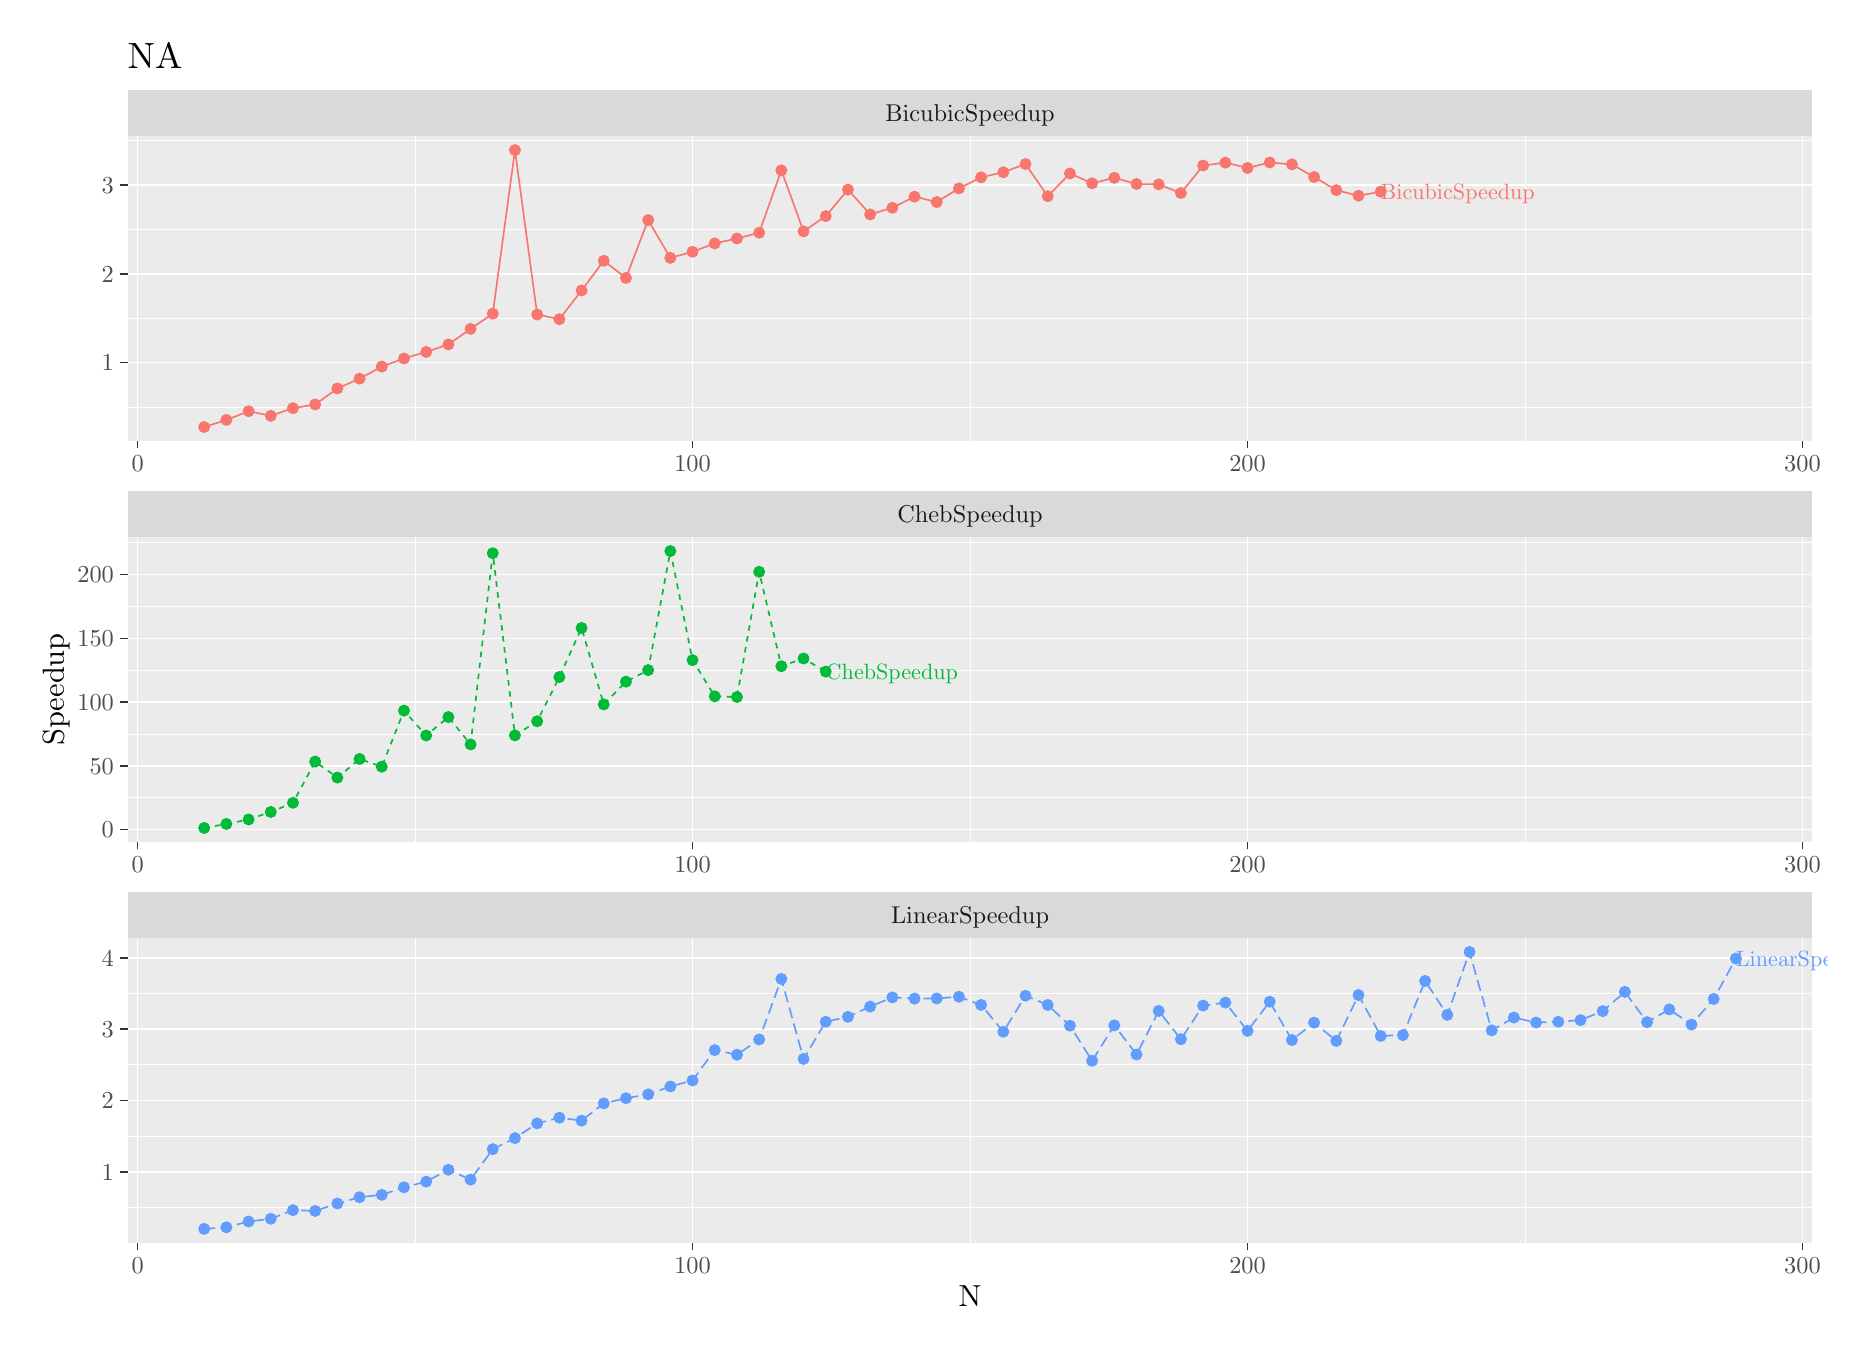
\begin{tikzpicture}[x=1pt,y=1pt]
\definecolor{fillColor}{RGB}{255,255,255}
\path[use as bounding box,fill=fillColor,fill opacity=0.00] (0,0) rectangle (650.43,469.76);
\begin{scope}
\path[clip] (  0.00,  0.00) rectangle (650.43,469.75);
\definecolor{drawColor}{RGB}{255,255,255}
\definecolor{fillColor}{RGB}{255,255,255}

\path[draw=drawColor,line width= 0.6pt,line join=round,line cap=round,fill=fillColor] (  0.00,  0.00) rectangle (650.43,469.75);
\end{scope}
\begin{scope}
\path[clip] (  0.00,  0.00) rectangle (650.43,469.76);
\definecolor{fillColor}{gray}{0.92}

\path[fill=fillColor] ( 36.11,320.44) rectangle (644.93,430.53);
\definecolor{drawColor}{RGB}{255,255,255}

\path[draw=drawColor,line width= 0.3pt,line join=round] ( 36.11,332.69) --
	(644.93,332.69);

\path[draw=drawColor,line width= 0.3pt,line join=round] ( 36.11,364.78) --
	(644.93,364.78);

\path[draw=drawColor,line width= 0.3pt,line join=round] ( 36.11,396.87) --
	(644.93,396.87);

\path[draw=drawColor,line width= 0.3pt,line join=round] ( 36.11,428.96) --
	(644.93,428.96);

\path[draw=drawColor,line width= 0.3pt,line join=round] (139.99,320.44) --
	(139.99,430.53);

\path[draw=drawColor,line width= 0.3pt,line join=round] (340.52,320.44) --
	(340.52,430.53);

\path[draw=drawColor,line width= 0.3pt,line join=round] (541.05,320.44) --
	(541.05,430.53);

\path[draw=drawColor,line width= 0.6pt,line join=round] ( 36.11,348.73) --
	(644.93,348.73);

\path[draw=drawColor,line width= 0.6pt,line join=round] ( 36.11,380.83) --
	(644.93,380.83);

\path[draw=drawColor,line width= 0.6pt,line join=round] ( 36.11,412.92) --
	(644.93,412.92);

\path[draw=drawColor,line width= 0.6pt,line join=round] ( 39.72,320.44) --
	( 39.72,430.53);

\path[draw=drawColor,line width= 0.6pt,line join=round] (240.25,320.44) --
	(240.25,430.53);

\path[draw=drawColor,line width= 0.6pt,line join=round] (440.79,320.44) --
	(440.79,430.53);

\path[draw=drawColor,line width= 0.6pt,line join=round] (641.32,320.44) --
	(641.32,430.53);
\definecolor{drawColor}{RGB}{248,118,109}

\path[draw=drawColor,line width= 0.6pt,line join=round] ( 63.78,325.45) --
	( 71.81,328.01) --
	( 79.83,331.17) --
	( 87.85,329.50) --
	( 95.87,332.26) --
	(103.89,333.60) --
	(111.91,339.38) --
	(119.93,342.92) --
	(127.96,347.28) --
	(135.98,350.23) --
	(144.00,352.58) --
	(152.02,355.29) --
	(160.04,360.91) --
	(168.06,366.41) --
	(176.08,425.52) --
	(184.10,366.10) --
	(192.13,364.43) --
	(200.15,374.79) --
	(208.17,385.52) --
	(216.19,379.31) --
	(224.21,400.24) --
	(232.23,386.57) --
	(240.25,388.77) --
	(248.28,391.80) --
	(256.30,393.57) --
	(264.32,395.66) --
	(272.34,418.19) --
	(280.36,396.16) --
	(288.38,401.65) --
	(296.40,411.25) --
	(304.42,402.28) --
	(312.45,404.67) --
	(320.47,408.70) --
	(328.49,406.74) --
	(336.51,411.67) --
	(344.53,415.68) --
	(352.55,417.51) --
	(360.57,420.48) --
	(368.60,408.84) --
	(376.62,417.06) --
	(384.64,413.52) --
	(392.66,415.50) --
	(400.68,413.26) --
	(408.70,413.13) --
	(416.72,410.00) --
	(424.74,419.94) --
	(432.77,420.98) --
	(440.79,419.07) --
	(448.81,421.04) --
	(456.83,420.35) --
	(464.85,415.80) --
	(472.87,411.04) --
	(480.89,409.02) --
	(488.92,410.49);
\definecolor{fillColor}{RGB}{248,118,109}

\path[draw=drawColor,line width= 0.4pt,line join=round,line cap=round,fill=fillColor] ( 63.78,325.45) circle (  1.96);

\path[draw=drawColor,line width= 0.4pt,line join=round,line cap=round,fill=fillColor] ( 71.81,328.01) circle (  1.96);

\path[draw=drawColor,line width= 0.4pt,line join=round,line cap=round,fill=fillColor] ( 79.83,331.17) circle (  1.96);

\path[draw=drawColor,line width= 0.4pt,line join=round,line cap=round,fill=fillColor] ( 87.85,329.50) circle (  1.96);

\path[draw=drawColor,line width= 0.4pt,line join=round,line cap=round,fill=fillColor] ( 95.87,332.26) circle (  1.96);

\path[draw=drawColor,line width= 0.4pt,line join=round,line cap=round,fill=fillColor] (103.89,333.60) circle (  1.96);

\path[draw=drawColor,line width= 0.4pt,line join=round,line cap=round,fill=fillColor] (111.91,339.38) circle (  1.96);

\path[draw=drawColor,line width= 0.4pt,line join=round,line cap=round,fill=fillColor] (119.93,342.92) circle (  1.96);

\path[draw=drawColor,line width= 0.4pt,line join=round,line cap=round,fill=fillColor] (127.96,347.28) circle (  1.96);

\path[draw=drawColor,line width= 0.4pt,line join=round,line cap=round,fill=fillColor] (135.98,350.23) circle (  1.96);

\path[draw=drawColor,line width= 0.4pt,line join=round,line cap=round,fill=fillColor] (144.00,352.58) circle (  1.96);

\path[draw=drawColor,line width= 0.4pt,line join=round,line cap=round,fill=fillColor] (152.02,355.29) circle (  1.96);

\path[draw=drawColor,line width= 0.4pt,line join=round,line cap=round,fill=fillColor] (160.04,360.91) circle (  1.96);

\path[draw=drawColor,line width= 0.4pt,line join=round,line cap=round,fill=fillColor] (168.06,366.41) circle (  1.96);

\path[draw=drawColor,line width= 0.4pt,line join=round,line cap=round,fill=fillColor] (176.08,425.52) circle (  1.96);

\path[draw=drawColor,line width= 0.4pt,line join=round,line cap=round,fill=fillColor] (184.10,366.10) circle (  1.96);

\path[draw=drawColor,line width= 0.4pt,line join=round,line cap=round,fill=fillColor] (192.13,364.43) circle (  1.96);

\path[draw=drawColor,line width= 0.4pt,line join=round,line cap=round,fill=fillColor] (200.15,374.79) circle (  1.96);

\path[draw=drawColor,line width= 0.4pt,line join=round,line cap=round,fill=fillColor] (208.17,385.52) circle (  1.96);

\path[draw=drawColor,line width= 0.4pt,line join=round,line cap=round,fill=fillColor] (216.19,379.31) circle (  1.96);

\path[draw=drawColor,line width= 0.4pt,line join=round,line cap=round,fill=fillColor] (224.21,400.24) circle (  1.96);

\path[draw=drawColor,line width= 0.4pt,line join=round,line cap=round,fill=fillColor] (232.23,386.57) circle (  1.96);

\path[draw=drawColor,line width= 0.4pt,line join=round,line cap=round,fill=fillColor] (240.25,388.77) circle (  1.96);

\path[draw=drawColor,line width= 0.4pt,line join=round,line cap=round,fill=fillColor] (248.28,391.80) circle (  1.96);

\path[draw=drawColor,line width= 0.4pt,line join=round,line cap=round,fill=fillColor] (256.30,393.57) circle (  1.96);

\path[draw=drawColor,line width= 0.4pt,line join=round,line cap=round,fill=fillColor] (264.32,395.66) circle (  1.96);

\path[draw=drawColor,line width= 0.4pt,line join=round,line cap=round,fill=fillColor] (272.34,418.19) circle (  1.96);

\path[draw=drawColor,line width= 0.4pt,line join=round,line cap=round,fill=fillColor] (280.36,396.16) circle (  1.96);

\path[draw=drawColor,line width= 0.4pt,line join=round,line cap=round,fill=fillColor] (288.38,401.65) circle (  1.96);

\path[draw=drawColor,line width= 0.4pt,line join=round,line cap=round,fill=fillColor] (296.40,411.25) circle (  1.96);

\path[draw=drawColor,line width= 0.4pt,line join=round,line cap=round,fill=fillColor] (304.42,402.28) circle (  1.96);

\path[draw=drawColor,line width= 0.4pt,line join=round,line cap=round,fill=fillColor] (312.45,404.67) circle (  1.96);

\path[draw=drawColor,line width= 0.4pt,line join=round,line cap=round,fill=fillColor] (320.47,408.70) circle (  1.96);

\path[draw=drawColor,line width= 0.4pt,line join=round,line cap=round,fill=fillColor] (328.49,406.74) circle (  1.96);

\path[draw=drawColor,line width= 0.4pt,line join=round,line cap=round,fill=fillColor] (336.51,411.67) circle (  1.96);

\path[draw=drawColor,line width= 0.4pt,line join=round,line cap=round,fill=fillColor] (344.53,415.68) circle (  1.96);

\path[draw=drawColor,line width= 0.4pt,line join=round,line cap=round,fill=fillColor] (352.55,417.51) circle (  1.96);

\path[draw=drawColor,line width= 0.4pt,line join=round,line cap=round,fill=fillColor] (360.57,420.48) circle (  1.96);

\path[draw=drawColor,line width= 0.4pt,line join=round,line cap=round,fill=fillColor] (368.60,408.84) circle (  1.96);

\path[draw=drawColor,line width= 0.4pt,line join=round,line cap=round,fill=fillColor] (376.62,417.06) circle (  1.96);

\path[draw=drawColor,line width= 0.4pt,line join=round,line cap=round,fill=fillColor] (384.64,413.52) circle (  1.96);

\path[draw=drawColor,line width= 0.4pt,line join=round,line cap=round,fill=fillColor] (392.66,415.50) circle (  1.96);

\path[draw=drawColor,line width= 0.4pt,line join=round,line cap=round,fill=fillColor] (400.68,413.26) circle (  1.96);

\path[draw=drawColor,line width= 0.4pt,line join=round,line cap=round,fill=fillColor] (408.70,413.13) circle (  1.96);

\path[draw=drawColor,line width= 0.4pt,line join=round,line cap=round,fill=fillColor] (416.72,410.00) circle (  1.96);

\path[draw=drawColor,line width= 0.4pt,line join=round,line cap=round,fill=fillColor] (424.74,419.94) circle (  1.96);

\path[draw=drawColor,line width= 0.4pt,line join=round,line cap=round,fill=fillColor] (432.77,420.98) circle (  1.96);

\path[draw=drawColor,line width= 0.4pt,line join=round,line cap=round,fill=fillColor] (440.79,419.07) circle (  1.96);

\path[draw=drawColor,line width= 0.4pt,line join=round,line cap=round,fill=fillColor] (448.81,421.04) circle (  1.96);

\path[draw=drawColor,line width= 0.4pt,line join=round,line cap=round,fill=fillColor] (456.83,420.35) circle (  1.96);

\path[draw=drawColor,line width= 0.4pt,line join=round,line cap=round,fill=fillColor] (464.85,415.80) circle (  1.96);

\path[draw=drawColor,line width= 0.4pt,line join=round,line cap=round,fill=fillColor] (472.87,411.04) circle (  1.96);

\path[draw=drawColor,line width= 0.4pt,line join=round,line cap=round,fill=fillColor] (480.89,409.02) circle (  1.96);

\path[draw=drawColor,line width= 0.4pt,line join=round,line cap=round,fill=fillColor] (488.92,410.49) circle (  1.96);

\node[text=drawColor,anchor=base west,inner sep=0pt, outer sep=0pt, scale=  0.80] at (488.92,407.74) {BicubicSpeedup};
\end{scope}
\begin{scope}
\path[clip] (  0.00,  0.00) rectangle (650.43,469.76);
\definecolor{fillColor}{gray}{0.92}

\path[fill=fillColor] ( 36.11,175.56) rectangle (644.93,285.65);
\definecolor{drawColor}{RGB}{255,255,255}

\path[draw=drawColor,line width= 0.3pt,line join=round] ( 36.11,191.50) --
	(644.93,191.50);

\path[draw=drawColor,line width= 0.3pt,line join=round] ( 36.11,214.54) --
	(644.93,214.54);

\path[draw=drawColor,line width= 0.3pt,line join=round] ( 36.11,237.57) --
	(644.93,237.57);

\path[draw=drawColor,line width= 0.3pt,line join=round] ( 36.11,260.61) --
	(644.93,260.61);

\path[draw=drawColor,line width= 0.3pt,line join=round] ( 36.11,283.65) --
	(644.93,283.65);

\path[draw=drawColor,line width= 0.3pt,line join=round] (139.99,175.56) --
	(139.99,285.65);

\path[draw=drawColor,line width= 0.3pt,line join=round] (340.52,175.56) --
	(340.52,285.65);

\path[draw=drawColor,line width= 0.3pt,line join=round] (541.05,175.56) --
	(541.05,285.65);

\path[draw=drawColor,line width= 0.6pt,line join=round] ( 36.11,179.98) --
	(644.93,179.98);

\path[draw=drawColor,line width= 0.6pt,line join=round] ( 36.11,203.02) --
	(644.93,203.02);

\path[draw=drawColor,line width= 0.6pt,line join=round] ( 36.11,226.05) --
	(644.93,226.05);

\path[draw=drawColor,line width= 0.6pt,line join=round] ( 36.11,249.09) --
	(644.93,249.09);

\path[draw=drawColor,line width= 0.6pt,line join=round] ( 36.11,272.13) --
	(644.93,272.13);

\path[draw=drawColor,line width= 0.6pt,line join=round] ( 39.72,175.56) --
	( 39.72,285.65);

\path[draw=drawColor,line width= 0.6pt,line join=round] (240.25,175.56) --
	(240.25,285.65);

\path[draw=drawColor,line width= 0.6pt,line join=round] (440.79,175.56) --
	(440.79,285.65);

\path[draw=drawColor,line width= 0.6pt,line join=round] (641.32,175.56) --
	(641.32,285.65);
\definecolor{drawColor}{RGB}{0,186,56}

\path[draw=drawColor,line width= 0.6pt,dash pattern=on 2pt off 2pt ,line join=round] ( 63.78,180.57) --
	( 71.81,182.02) --
	( 79.83,183.64) --
	( 87.85,186.35) --
	( 95.87,189.66) --
	(103.89,204.56) --
	(111.91,198.78) --
	(119.93,205.50) --
	(127.96,202.71) --
	(135.98,222.97) --
	(144.00,213.99) --
	(152.02,220.65) --
	(160.04,210.76) --
	(168.06,279.86) --
	(176.08,214.03) --
	(184.10,219.13) --
	(192.13,235.12) --
	(200.15,252.84) --
	(208.17,225.21) --
	(216.19,233.44) --
	(224.21,237.62) --
	(232.23,280.64) --
	(240.25,241.22) --
	(248.28,228.13) --
	(256.30,227.90) --
	(264.32,273.14) --
	(272.34,239.02) --
	(280.36,241.81) --
	(288.38,237.08);
\definecolor{fillColor}{RGB}{0,186,56}

\path[draw=drawColor,line width= 0.4pt,line join=round,line cap=round,fill=fillColor] ( 63.78,180.57) circle (  1.96);

\path[draw=drawColor,line width= 0.4pt,line join=round,line cap=round,fill=fillColor] ( 71.81,182.02) circle (  1.96);

\path[draw=drawColor,line width= 0.4pt,line join=round,line cap=round,fill=fillColor] ( 79.83,183.64) circle (  1.96);

\path[draw=drawColor,line width= 0.4pt,line join=round,line cap=round,fill=fillColor] ( 87.85,186.35) circle (  1.96);

\path[draw=drawColor,line width= 0.4pt,line join=round,line cap=round,fill=fillColor] ( 95.87,189.66) circle (  1.96);

\path[draw=drawColor,line width= 0.4pt,line join=round,line cap=round,fill=fillColor] (103.89,204.56) circle (  1.96);

\path[draw=drawColor,line width= 0.4pt,line join=round,line cap=round,fill=fillColor] (111.91,198.78) circle (  1.96);

\path[draw=drawColor,line width= 0.4pt,line join=round,line cap=round,fill=fillColor] (119.93,205.50) circle (  1.96);

\path[draw=drawColor,line width= 0.4pt,line join=round,line cap=round,fill=fillColor] (127.96,202.71) circle (  1.96);

\path[draw=drawColor,line width= 0.4pt,line join=round,line cap=round,fill=fillColor] (135.98,222.97) circle (  1.96);

\path[draw=drawColor,line width= 0.4pt,line join=round,line cap=round,fill=fillColor] (144.00,213.99) circle (  1.96);

\path[draw=drawColor,line width= 0.4pt,line join=round,line cap=round,fill=fillColor] (152.02,220.65) circle (  1.96);

\path[draw=drawColor,line width= 0.4pt,line join=round,line cap=round,fill=fillColor] (160.04,210.76) circle (  1.96);

\path[draw=drawColor,line width= 0.4pt,line join=round,line cap=round,fill=fillColor] (168.06,279.86) circle (  1.96);

\path[draw=drawColor,line width= 0.4pt,line join=round,line cap=round,fill=fillColor] (176.08,214.03) circle (  1.96);

\path[draw=drawColor,line width= 0.4pt,line join=round,line cap=round,fill=fillColor] (184.10,219.13) circle (  1.96);

\path[draw=drawColor,line width= 0.4pt,line join=round,line cap=round,fill=fillColor] (192.13,235.12) circle (  1.96);

\path[draw=drawColor,line width= 0.4pt,line join=round,line cap=round,fill=fillColor] (200.15,252.84) circle (  1.96);

\path[draw=drawColor,line width= 0.4pt,line join=round,line cap=round,fill=fillColor] (208.17,225.21) circle (  1.96);

\path[draw=drawColor,line width= 0.4pt,line join=round,line cap=round,fill=fillColor] (216.19,233.44) circle (  1.96);

\path[draw=drawColor,line width= 0.4pt,line join=round,line cap=round,fill=fillColor] (224.21,237.62) circle (  1.96);

\path[draw=drawColor,line width= 0.4pt,line join=round,line cap=round,fill=fillColor] (232.23,280.64) circle (  1.96);

\path[draw=drawColor,line width= 0.4pt,line join=round,line cap=round,fill=fillColor] (240.25,241.22) circle (  1.96);

\path[draw=drawColor,line width= 0.4pt,line join=round,line cap=round,fill=fillColor] (248.28,228.13) circle (  1.96);

\path[draw=drawColor,line width= 0.4pt,line join=round,line cap=round,fill=fillColor] (256.30,227.90) circle (  1.96);

\path[draw=drawColor,line width= 0.4pt,line join=round,line cap=round,fill=fillColor] (264.32,273.14) circle (  1.96);

\path[draw=drawColor,line width= 0.4pt,line join=round,line cap=round,fill=fillColor] (272.34,239.02) circle (  1.96);

\path[draw=drawColor,line width= 0.4pt,line join=round,line cap=round,fill=fillColor] (280.36,241.81) circle (  1.96);

\path[draw=drawColor,line width= 0.4pt,line join=round,line cap=round,fill=fillColor] (288.38,237.08) circle (  1.96);

\node[text=drawColor,anchor=base west,inner sep=0pt, outer sep=0pt, scale=  0.80] at (288.38,234.33) {ChebSpeedup};
\end{scope}
\begin{scope}
\path[clip] (  0.00,  0.00) rectangle (650.43,469.76);
\definecolor{fillColor}{gray}{0.92}

\path[fill=fillColor] ( 36.11, 30.69) rectangle (644.93,140.77);
\definecolor{drawColor}{RGB}{255,255,255}

\path[draw=drawColor,line width= 0.3pt,line join=round] ( 36.11, 43.50) --
	(644.93, 43.50);

\path[draw=drawColor,line width= 0.3pt,line join=round] ( 36.11, 69.24) --
	(644.93, 69.24);

\path[draw=drawColor,line width= 0.3pt,line join=round] ( 36.11, 94.97) --
	(644.93, 94.97);

\path[draw=drawColor,line width= 0.3pt,line join=round] ( 36.11,120.71) --
	(644.93,120.71);

\path[draw=drawColor,line width= 0.3pt,line join=round] (139.99, 30.69) --
	(139.99,140.77);

\path[draw=drawColor,line width= 0.3pt,line join=round] (340.52, 30.69) --
	(340.52,140.77);

\path[draw=drawColor,line width= 0.3pt,line join=round] (541.05, 30.69) --
	(541.05,140.77);

\path[draw=drawColor,line width= 0.6pt,line join=round] ( 36.11, 56.37) --
	(644.93, 56.37);

\path[draw=drawColor,line width= 0.6pt,line join=round] ( 36.11, 82.10) --
	(644.93, 82.10);

\path[draw=drawColor,line width= 0.6pt,line join=round] ( 36.11,107.84) --
	(644.93,107.84);

\path[draw=drawColor,line width= 0.6pt,line join=round] ( 36.11,133.58) --
	(644.93,133.58);

\path[draw=drawColor,line width= 0.6pt,line join=round] ( 39.72, 30.69) --
	( 39.72,140.77);

\path[draw=drawColor,line width= 0.6pt,line join=round] (240.25, 30.69) --
	(240.25,140.77);

\path[draw=drawColor,line width= 0.6pt,line join=round] (440.79, 30.69) --
	(440.79,140.77);

\path[draw=drawColor,line width= 0.6pt,line join=round] (641.32, 30.69) --
	(641.32,140.77);
\definecolor{drawColor}{RGB}{97,156,255}

\path[draw=drawColor,line width= 0.6pt,dash pattern=on 4pt off 2pt ,line join=round] ( 63.78, 35.69) --
	( 71.81, 36.27) --
	( 79.83, 38.36) --
	( 87.85, 39.36) --
	( 95.87, 42.47) --
	(103.89, 42.19) --
	(111.91, 44.89) --
	(119.93, 47.15) --
	(127.96, 48.01) --
	(135.98, 50.72) --
	(144.00, 52.77) --
	(152.02, 57.07) --
	(160.04, 53.49) --
	(168.06, 64.51) --
	(176.08, 68.50) --
	(184.10, 73.81) --
	(192.13, 75.87) --
	(200.15, 74.82) --
	(208.17, 81.05) --
	(216.19, 82.92) --
	(224.21, 84.31) --
	(232.23, 87.16) --
	(240.25, 89.34) --
	(248.28,100.31) --
	(256.30, 98.64) --
	(264.32,104.13) --
	(272.34,126.02) --
	(280.36, 97.12) --
	(288.38,110.55) --
	(296.40,112.32) --
	(304.42,116.03) --
	(312.45,119.34) --
	(320.47,118.91) --
	(328.49,118.97) --
	(336.51,119.58) --
	(344.53,116.63) --
	(352.55,106.93) --
	(360.57,119.95) --
	(368.60,116.61) --
	(376.62,109.12) --
	(384.64, 96.44) --
	(392.66,109.23) --
	(400.68, 98.73) --
	(408.70,114.46) --
	(416.72,104.24) --
	(424.74,116.39) --
	(432.77,117.46) --
	(440.79,107.27) --
	(448.81,117.80) --
	(456.83,103.95) --
	(464.85,110.23) --
	(472.87,103.63) --
	(480.89,120.19) --
	(488.92,105.42) --
	(496.94,105.73) --
	(504.96,125.30) --
	(512.98,113.04) --
	(521.00,135.77) --
	(529.02,107.44) --
	(537.04,112.06) --
	(545.06,110.27) --
	(553.09,110.54) --
	(561.11,111.14) --
	(569.13,114.38) --
	(577.15,121.34) --
	(585.17,110.40) --
	(593.19,115.01) --
	(601.21,109.53) --
	(609.24,118.79) --
	(617.26,133.39);
\definecolor{fillColor}{RGB}{97,156,255}

\path[draw=drawColor,line width= 0.4pt,line join=round,line cap=round,fill=fillColor] ( 63.78, 35.69) circle (  1.96);

\path[draw=drawColor,line width= 0.4pt,line join=round,line cap=round,fill=fillColor] ( 71.81, 36.27) circle (  1.96);

\path[draw=drawColor,line width= 0.4pt,line join=round,line cap=round,fill=fillColor] ( 79.83, 38.36) circle (  1.96);

\path[draw=drawColor,line width= 0.4pt,line join=round,line cap=round,fill=fillColor] ( 87.85, 39.36) circle (  1.96);

\path[draw=drawColor,line width= 0.4pt,line join=round,line cap=round,fill=fillColor] ( 95.87, 42.47) circle (  1.96);

\path[draw=drawColor,line width= 0.4pt,line join=round,line cap=round,fill=fillColor] (103.89, 42.19) circle (  1.96);

\path[draw=drawColor,line width= 0.4pt,line join=round,line cap=round,fill=fillColor] (111.91, 44.89) circle (  1.96);

\path[draw=drawColor,line width= 0.4pt,line join=round,line cap=round,fill=fillColor] (119.93, 47.15) circle (  1.96);

\path[draw=drawColor,line width= 0.4pt,line join=round,line cap=round,fill=fillColor] (127.96, 48.01) circle (  1.96);

\path[draw=drawColor,line width= 0.4pt,line join=round,line cap=round,fill=fillColor] (135.98, 50.72) circle (  1.96);

\path[draw=drawColor,line width= 0.4pt,line join=round,line cap=round,fill=fillColor] (144.00, 52.77) circle (  1.96);

\path[draw=drawColor,line width= 0.4pt,line join=round,line cap=round,fill=fillColor] (152.02, 57.07) circle (  1.96);

\path[draw=drawColor,line width= 0.4pt,line join=round,line cap=round,fill=fillColor] (160.04, 53.49) circle (  1.96);

\path[draw=drawColor,line width= 0.4pt,line join=round,line cap=round,fill=fillColor] (168.06, 64.51) circle (  1.96);

\path[draw=drawColor,line width= 0.4pt,line join=round,line cap=round,fill=fillColor] (176.08, 68.50) circle (  1.96);

\path[draw=drawColor,line width= 0.4pt,line join=round,line cap=round,fill=fillColor] (184.10, 73.81) circle (  1.96);

\path[draw=drawColor,line width= 0.4pt,line join=round,line cap=round,fill=fillColor] (192.13, 75.87) circle (  1.96);

\path[draw=drawColor,line width= 0.4pt,line join=round,line cap=round,fill=fillColor] (200.15, 74.82) circle (  1.96);

\path[draw=drawColor,line width= 0.4pt,line join=round,line cap=round,fill=fillColor] (208.17, 81.05) circle (  1.96);

\path[draw=drawColor,line width= 0.4pt,line join=round,line cap=round,fill=fillColor] (216.19, 82.92) circle (  1.96);

\path[draw=drawColor,line width= 0.4pt,line join=round,line cap=round,fill=fillColor] (224.21, 84.31) circle (  1.96);

\path[draw=drawColor,line width= 0.4pt,line join=round,line cap=round,fill=fillColor] (232.23, 87.16) circle (  1.96);

\path[draw=drawColor,line width= 0.4pt,line join=round,line cap=round,fill=fillColor] (240.25, 89.34) circle (  1.96);

\path[draw=drawColor,line width= 0.4pt,line join=round,line cap=round,fill=fillColor] (248.28,100.31) circle (  1.96);

\path[draw=drawColor,line width= 0.4pt,line join=round,line cap=round,fill=fillColor] (256.30, 98.64) circle (  1.96);

\path[draw=drawColor,line width= 0.4pt,line join=round,line cap=round,fill=fillColor] (264.32,104.13) circle (  1.96);

\path[draw=drawColor,line width= 0.4pt,line join=round,line cap=round,fill=fillColor] (272.34,126.02) circle (  1.96);

\path[draw=drawColor,line width= 0.4pt,line join=round,line cap=round,fill=fillColor] (280.36, 97.12) circle (  1.96);

\path[draw=drawColor,line width= 0.4pt,line join=round,line cap=round,fill=fillColor] (288.38,110.55) circle (  1.96);

\path[draw=drawColor,line width= 0.4pt,line join=round,line cap=round,fill=fillColor] (296.40,112.32) circle (  1.96);

\path[draw=drawColor,line width= 0.4pt,line join=round,line cap=round,fill=fillColor] (304.42,116.03) circle (  1.96);

\path[draw=drawColor,line width= 0.4pt,line join=round,line cap=round,fill=fillColor] (312.45,119.34) circle (  1.96);

\path[draw=drawColor,line width= 0.4pt,line join=round,line cap=round,fill=fillColor] (320.47,118.91) circle (  1.96);

\path[draw=drawColor,line width= 0.4pt,line join=round,line cap=round,fill=fillColor] (328.49,118.97) circle (  1.96);

\path[draw=drawColor,line width= 0.4pt,line join=round,line cap=round,fill=fillColor] (336.51,119.58) circle (  1.96);

\path[draw=drawColor,line width= 0.4pt,line join=round,line cap=round,fill=fillColor] (344.53,116.63) circle (  1.96);

\path[draw=drawColor,line width= 0.4pt,line join=round,line cap=round,fill=fillColor] (352.55,106.93) circle (  1.96);

\path[draw=drawColor,line width= 0.4pt,line join=round,line cap=round,fill=fillColor] (360.57,119.95) circle (  1.96);

\path[draw=drawColor,line width= 0.4pt,line join=round,line cap=round,fill=fillColor] (368.60,116.61) circle (  1.96);

\path[draw=drawColor,line width= 0.4pt,line join=round,line cap=round,fill=fillColor] (376.62,109.12) circle (  1.96);

\path[draw=drawColor,line width= 0.4pt,line join=round,line cap=round,fill=fillColor] (384.64, 96.44) circle (  1.96);

\path[draw=drawColor,line width= 0.4pt,line join=round,line cap=round,fill=fillColor] (392.66,109.23) circle (  1.96);

\path[draw=drawColor,line width= 0.4pt,line join=round,line cap=round,fill=fillColor] (400.68, 98.73) circle (  1.96);

\path[draw=drawColor,line width= 0.4pt,line join=round,line cap=round,fill=fillColor] (408.70,114.46) circle (  1.96);

\path[draw=drawColor,line width= 0.4pt,line join=round,line cap=round,fill=fillColor] (416.72,104.24) circle (  1.96);

\path[draw=drawColor,line width= 0.4pt,line join=round,line cap=round,fill=fillColor] (424.74,116.39) circle (  1.96);

\path[draw=drawColor,line width= 0.4pt,line join=round,line cap=round,fill=fillColor] (432.77,117.46) circle (  1.96);

\path[draw=drawColor,line width= 0.4pt,line join=round,line cap=round,fill=fillColor] (440.79,107.27) circle (  1.96);

\path[draw=drawColor,line width= 0.4pt,line join=round,line cap=round,fill=fillColor] (448.81,117.80) circle (  1.96);

\path[draw=drawColor,line width= 0.4pt,line join=round,line cap=round,fill=fillColor] (456.83,103.95) circle (  1.96);

\path[draw=drawColor,line width= 0.4pt,line join=round,line cap=round,fill=fillColor] (464.85,110.23) circle (  1.96);

\path[draw=drawColor,line width= 0.4pt,line join=round,line cap=round,fill=fillColor] (472.87,103.63) circle (  1.96);

\path[draw=drawColor,line width= 0.4pt,line join=round,line cap=round,fill=fillColor] (480.89,120.19) circle (  1.96);

\path[draw=drawColor,line width= 0.4pt,line join=round,line cap=round,fill=fillColor] (488.92,105.42) circle (  1.96);

\path[draw=drawColor,line width= 0.4pt,line join=round,line cap=round,fill=fillColor] (496.94,105.73) circle (  1.96);

\path[draw=drawColor,line width= 0.4pt,line join=round,line cap=round,fill=fillColor] (504.96,125.30) circle (  1.96);

\path[draw=drawColor,line width= 0.4pt,line join=round,line cap=round,fill=fillColor] (512.98,113.04) circle (  1.96);

\path[draw=drawColor,line width= 0.4pt,line join=round,line cap=round,fill=fillColor] (521.00,135.77) circle (  1.96);

\path[draw=drawColor,line width= 0.4pt,line join=round,line cap=round,fill=fillColor] (529.02,107.44) circle (  1.96);

\path[draw=drawColor,line width= 0.4pt,line join=round,line cap=round,fill=fillColor] (537.04,112.06) circle (  1.96);

\path[draw=drawColor,line width= 0.4pt,line join=round,line cap=round,fill=fillColor] (545.06,110.27) circle (  1.96);

\path[draw=drawColor,line width= 0.4pt,line join=round,line cap=round,fill=fillColor] (553.09,110.54) circle (  1.96);

\path[draw=drawColor,line width= 0.4pt,line join=round,line cap=round,fill=fillColor] (561.11,111.14) circle (  1.96);

\path[draw=drawColor,line width= 0.4pt,line join=round,line cap=round,fill=fillColor] (569.13,114.38) circle (  1.96);

\path[draw=drawColor,line width= 0.4pt,line join=round,line cap=round,fill=fillColor] (577.15,121.34) circle (  1.96);

\path[draw=drawColor,line width= 0.4pt,line join=round,line cap=round,fill=fillColor] (585.17,110.40) circle (  1.96);

\path[draw=drawColor,line width= 0.4pt,line join=round,line cap=round,fill=fillColor] (593.19,115.01) circle (  1.96);

\path[draw=drawColor,line width= 0.4pt,line join=round,line cap=round,fill=fillColor] (601.21,109.53) circle (  1.96);

\path[draw=drawColor,line width= 0.4pt,line join=round,line cap=round,fill=fillColor] (609.24,118.79) circle (  1.96);

\path[draw=drawColor,line width= 0.4pt,line join=round,line cap=round,fill=fillColor] (617.26,133.39) circle (  1.96);

\node[text=drawColor,anchor=base west,inner sep=0pt, outer sep=0pt, scale=  0.80] at (617.26,130.63) {LinearSpeedup};
\end{scope}
\begin{scope}
\path[clip] ( 36.11,140.77) rectangle (644.93,157.34);
\definecolor{fillColor}{gray}{0.85}

\path[fill=fillColor] ( 36.11,140.77) rectangle (644.93,157.34);
\definecolor{drawColor}{gray}{0.10}

\node[text=drawColor,anchor=base,inner sep=0pt, outer sep=0pt, scale=  0.88] at (340.52,146.03) {LinearSpeedup};
\end{scope}
\begin{scope}
\path[clip] ( 36.11,285.65) rectangle (644.93,302.22);
\definecolor{fillColor}{gray}{0.85}

\path[fill=fillColor] ( 36.11,285.65) rectangle (644.93,302.22);
\definecolor{drawColor}{gray}{0.10}

\node[text=drawColor,anchor=base,inner sep=0pt, outer sep=0pt, scale=  0.88] at (340.52,290.90) {ChebSpeedup};
\end{scope}
\begin{scope}
\path[clip] ( 36.11,430.53) rectangle (644.93,447.10);
\definecolor{fillColor}{gray}{0.85}

\path[fill=fillColor] ( 36.11,430.53) rectangle (644.93,447.10);
\definecolor{drawColor}{gray}{0.10}

\node[text=drawColor,anchor=base,inner sep=0pt, outer sep=0pt, scale=  0.88] at (340.52,435.78) {BicubicSpeedup};
\end{scope}
\begin{scope}
\path[clip] (  0.00,  0.00) rectangle (650.43,469.76);
\definecolor{drawColor}{gray}{0.20}

\path[draw=drawColor,line width= 0.6pt,line join=round] ( 39.72, 27.94) --
	( 39.72, 30.69);

\path[draw=drawColor,line width= 0.6pt,line join=round] (240.25, 27.94) --
	(240.25, 30.69);

\path[draw=drawColor,line width= 0.6pt,line join=round] (440.79, 27.94) --
	(440.79, 30.69);

\path[draw=drawColor,line width= 0.6pt,line join=round] (641.32, 27.94) --
	(641.32, 30.69);
\end{scope}
\begin{scope}
\path[clip] (  0.00,  0.00) rectangle (650.43,469.76);
\definecolor{drawColor}{gray}{0.30}

\node[text=drawColor,anchor=base,inner sep=0pt, outer sep=0pt, scale=  0.88] at ( 39.72, 19.68) {0};

\node[text=drawColor,anchor=base,inner sep=0pt, outer sep=0pt, scale=  0.88] at (240.25, 19.68) {100};

\node[text=drawColor,anchor=base,inner sep=0pt, outer sep=0pt, scale=  0.88] at (440.79, 19.68) {200};

\node[text=drawColor,anchor=base,inner sep=0pt, outer sep=0pt, scale=  0.88] at (641.32, 19.68) {300};
\end{scope}
\begin{scope}
\path[clip] (  0.00,  0.00) rectangle (650.43,469.76);
\definecolor{drawColor}{gray}{0.20}

\path[draw=drawColor,line width= 0.6pt,line join=round] ( 39.72,172.81) --
	( 39.72,175.56);

\path[draw=drawColor,line width= 0.6pt,line join=round] (240.25,172.81) --
	(240.25,175.56);

\path[draw=drawColor,line width= 0.6pt,line join=round] (440.79,172.81) --
	(440.79,175.56);

\path[draw=drawColor,line width= 0.6pt,line join=round] (641.32,172.81) --
	(641.32,175.56);
\end{scope}
\begin{scope}
\path[clip] (  0.00,  0.00) rectangle (650.43,469.76);
\definecolor{drawColor}{gray}{0.30}

\node[text=drawColor,anchor=base,inner sep=0pt, outer sep=0pt, scale=  0.88] at ( 39.72,164.55) {0};

\node[text=drawColor,anchor=base,inner sep=0pt, outer sep=0pt, scale=  0.88] at (240.25,164.55) {100};

\node[text=drawColor,anchor=base,inner sep=0pt, outer sep=0pt, scale=  0.88] at (440.79,164.55) {200};

\node[text=drawColor,anchor=base,inner sep=0pt, outer sep=0pt, scale=  0.88] at (641.32,164.55) {300};
\end{scope}
\begin{scope}
\path[clip] (  0.00,  0.00) rectangle (650.43,469.76);
\definecolor{drawColor}{gray}{0.20}

\path[draw=drawColor,line width= 0.6pt,line join=round] ( 39.72,317.69) --
	( 39.72,320.44);

\path[draw=drawColor,line width= 0.6pt,line join=round] (240.25,317.69) --
	(240.25,320.44);

\path[draw=drawColor,line width= 0.6pt,line join=round] (440.79,317.69) --
	(440.79,320.44);

\path[draw=drawColor,line width= 0.6pt,line join=round] (641.32,317.69) --
	(641.32,320.44);
\end{scope}
\begin{scope}
\path[clip] (  0.00,  0.00) rectangle (650.43,469.76);
\definecolor{drawColor}{gray}{0.30}

\node[text=drawColor,anchor=base,inner sep=0pt, outer sep=0pt, scale=  0.88] at ( 39.72,309.43) {0};

\node[text=drawColor,anchor=base,inner sep=0pt, outer sep=0pt, scale=  0.88] at (240.25,309.43) {100};

\node[text=drawColor,anchor=base,inner sep=0pt, outer sep=0pt, scale=  0.88] at (440.79,309.43) {200};

\node[text=drawColor,anchor=base,inner sep=0pt, outer sep=0pt, scale=  0.88] at (641.32,309.43) {300};
\end{scope}
\begin{scope}
\path[clip] (  0.00,  0.00) rectangle (650.43,469.76);
\definecolor{drawColor}{gray}{0.30}

\node[text=drawColor,anchor=base east,inner sep=0pt, outer sep=0pt, scale=  0.88] at ( 31.16,345.70) {1};

\node[text=drawColor,anchor=base east,inner sep=0pt, outer sep=0pt, scale=  0.88] at ( 31.16,377.79) {2};

\node[text=drawColor,anchor=base east,inner sep=0pt, outer sep=0pt, scale=  0.88] at ( 31.16,409.89) {3};
\end{scope}
\begin{scope}
\path[clip] (  0.00,  0.00) rectangle (650.43,469.76);
\definecolor{drawColor}{gray}{0.20}

\path[draw=drawColor,line width= 0.6pt,line join=round] ( 33.36,348.73) --
	( 36.11,348.73);

\path[draw=drawColor,line width= 0.6pt,line join=round] ( 33.36,380.83) --
	( 36.11,380.83);

\path[draw=drawColor,line width= 0.6pt,line join=round] ( 33.36,412.92) --
	( 36.11,412.92);
\end{scope}
\begin{scope}
\path[clip] (  0.00,  0.00) rectangle (650.43,469.76);
\definecolor{drawColor}{gray}{0.30}

\node[text=drawColor,anchor=base east,inner sep=0pt, outer sep=0pt, scale=  0.88] at ( 31.16,176.95) {0};

\node[text=drawColor,anchor=base east,inner sep=0pt, outer sep=0pt, scale=  0.88] at ( 31.16,199.99) {50};

\node[text=drawColor,anchor=base east,inner sep=0pt, outer sep=0pt, scale=  0.88] at ( 31.16,223.02) {100};

\node[text=drawColor,anchor=base east,inner sep=0pt, outer sep=0pt, scale=  0.88] at ( 31.16,246.06) {150};

\node[text=drawColor,anchor=base east,inner sep=0pt, outer sep=0pt, scale=  0.88] at ( 31.16,269.10) {200};
\end{scope}
\begin{scope}
\path[clip] (  0.00,  0.00) rectangle (650.43,469.76);
\definecolor{drawColor}{gray}{0.20}

\path[draw=drawColor,line width= 0.6pt,line join=round] ( 33.36,179.98) --
	( 36.11,179.98);

\path[draw=drawColor,line width= 0.6pt,line join=round] ( 33.36,203.02) --
	( 36.11,203.02);

\path[draw=drawColor,line width= 0.6pt,line join=round] ( 33.36,226.05) --
	( 36.11,226.05);

\path[draw=drawColor,line width= 0.6pt,line join=round] ( 33.36,249.09) --
	( 36.11,249.09);

\path[draw=drawColor,line width= 0.6pt,line join=round] ( 33.36,272.13) --
	( 36.11,272.13);
\end{scope}
\begin{scope}
\path[clip] (  0.00,  0.00) rectangle (650.43,469.76);
\definecolor{drawColor}{gray}{0.30}

\node[text=drawColor,anchor=base east,inner sep=0pt, outer sep=0pt, scale=  0.88] at ( 31.16, 53.34) {1};

\node[text=drawColor,anchor=base east,inner sep=0pt, outer sep=0pt, scale=  0.88] at ( 31.16, 79.07) {2};

\node[text=drawColor,anchor=base east,inner sep=0pt, outer sep=0pt, scale=  0.88] at ( 31.16,104.81) {3};

\node[text=drawColor,anchor=base east,inner sep=0pt, outer sep=0pt, scale=  0.88] at ( 31.16,130.55) {4};
\end{scope}
\begin{scope}
\path[clip] (  0.00,  0.00) rectangle (650.43,469.76);
\definecolor{drawColor}{gray}{0.20}

\path[draw=drawColor,line width= 0.6pt,line join=round] ( 33.36, 56.37) --
	( 36.11, 56.37);

\path[draw=drawColor,line width= 0.6pt,line join=round] ( 33.36, 82.10) --
	( 36.11, 82.10);

\path[draw=drawColor,line width= 0.6pt,line join=round] ( 33.36,107.84) --
	( 36.11,107.84);

\path[draw=drawColor,line width= 0.6pt,line join=round] ( 33.36,133.58) --
	( 36.11,133.58);
\end{scope}
\begin{scope}
\path[clip] (  0.00,  0.00) rectangle (650.43,469.76);
\definecolor{drawColor}{RGB}{0,0,0}

\node[text=drawColor,anchor=base,inner sep=0pt, outer sep=0pt, scale=  1.10] at (340.52,  7.64) {N};
\end{scope}
\begin{scope}
\path[clip] (  0.00,  0.00) rectangle (650.43,469.76);
\definecolor{drawColor}{RGB}{0,0,0}

\node[text=drawColor,rotate= 90.00,anchor=base,inner sep=0pt, outer sep=0pt, scale=  1.10] at ( 13.08,230.61) {Speedup};
\end{scope}
\begin{scope}
\path[clip] (  0.00,  0.00) rectangle (650.43,469.76);
\definecolor{drawColor}{RGB}{0,0,0}

\node[text=drawColor,anchor=base west,inner sep=0pt, outer sep=0pt, scale=  1.32] at ( 36.11,455.16) {NA};
\end{scope}
\end{tikzpicture}
